\documentclass[11pt,a4paper]{article}
\usepackage[utf8]{inputenc}
\usepackage{amsmath}
\usepackage{amsfonts}
\usepackage{amssymb}
\usepackage{graphicx}
\usepackage[affil-it]{authblk}

\begin{document}
\author{Jacob Bruner}
\title{MYP 2.1 - Pendulums}
\date{January 16th, 2021}
\affil{Advanced Algebra and Calculus I Honors \\ The Dwight School}
\maketitle
\tableofcontents
\pagebreak

\section{Problem Statement}

\begin{figure}[h]
\begin{center}
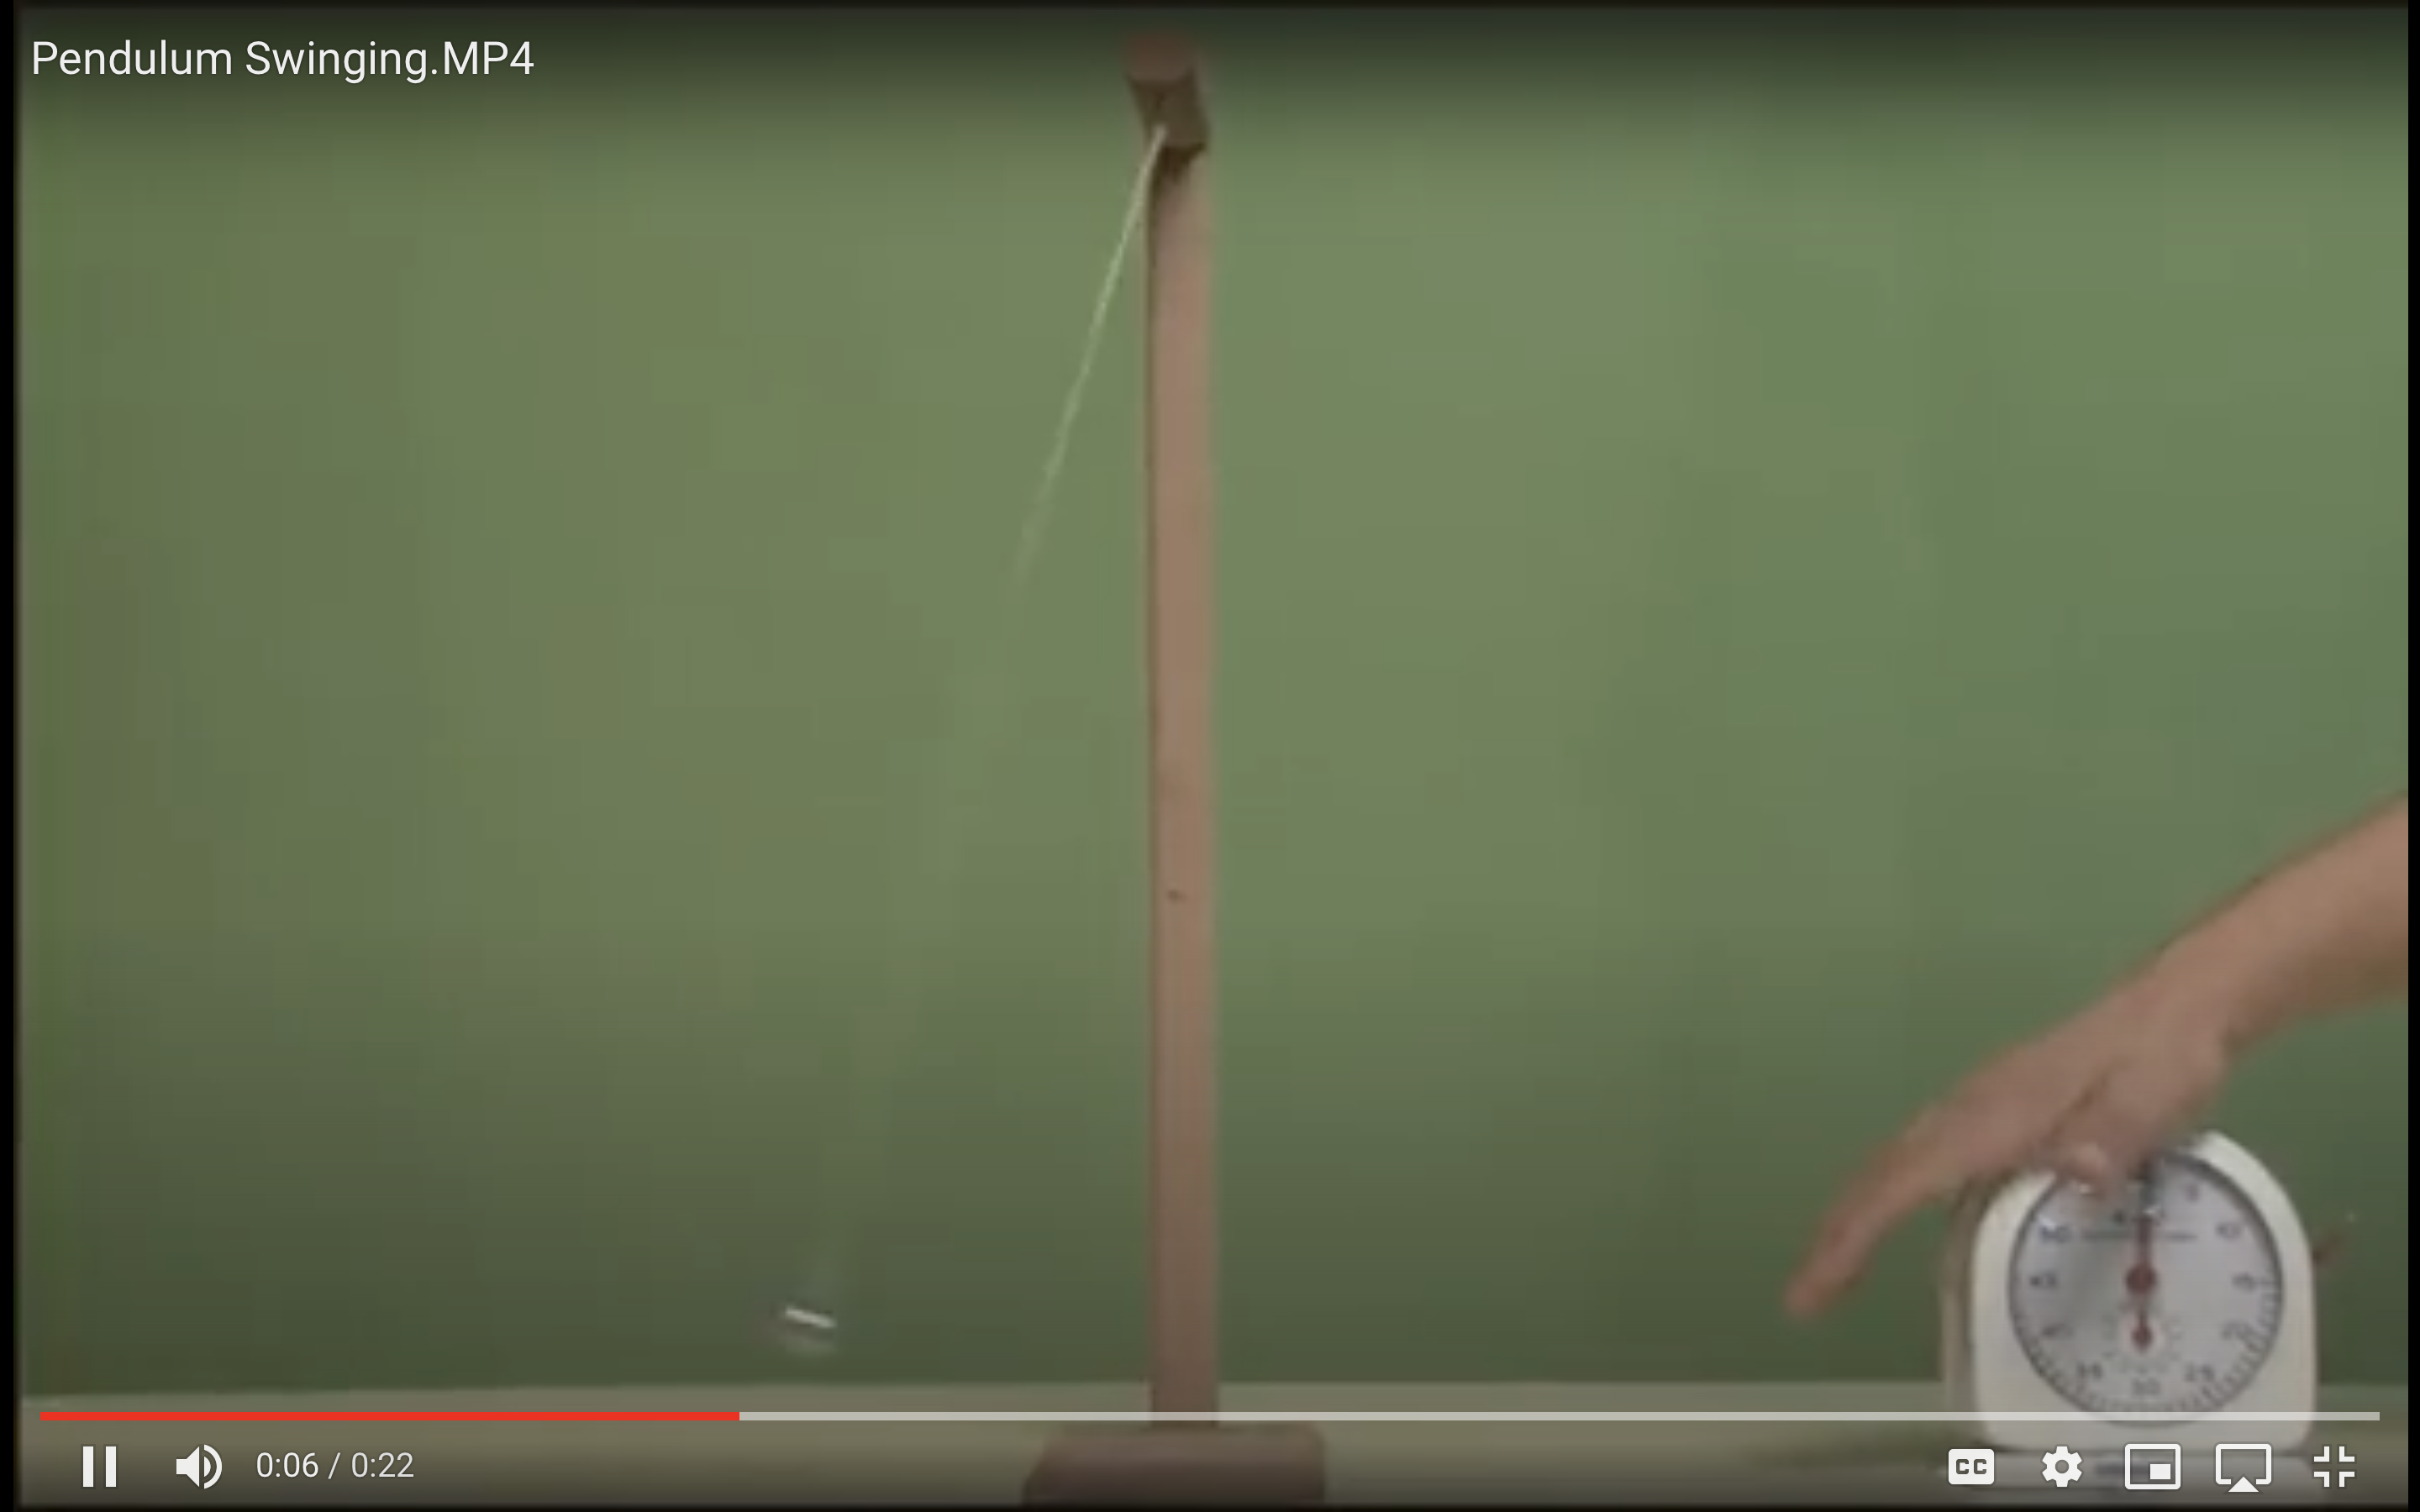
\includegraphics[scale=.24]{video.png} 
\caption{Video Provided}
\end{center}
\end{figure}


\subsection{Task}

Given a video of a pendulum swinging back and forth,  determine the the total approximate distance it will travel over the time period of one day.  Assume no-friction or drag forces.

\subsection{Required components}

The required component to determining the distance this pendulum would cover over a course of a day is the arclength of the sector formed by the maximum positions to the left and the right,  as well as the amount of time it takes for the pendulum to cover that distance.  These components can be determined in a number of ways,  but the most helpful physical properties unique to this pendulum include: radius from the center,  mass of the object,  gravitational force,  period,  and most notably the angle.  From these,  other components can be derived, such as restorative force,  angular velocity/ acceleration,  and tension force. \\
From the limited helpfulness of the video,  the given information is rather limited. No distance is directly given in the video,  so whatever method selected has to determine this.  My initial thoughts when given the video were "what will be the most accurate and feasible measurements I could make?" The option of comparing the size of other objects in the frame to the pendulum to determine distance was a possibility and I do believe it would yield a good degree of accuracy.  However,  I opted to measure the angle of the pendulum,  and the period of motion,  because I felt those would be the most accurate measurements I could make.
\section{Mathematical Model of a Pendulum}
\subsection{Accurate Model}
The accurate model of a pendulum in motion is a second-order differential equation derived from the principles of forces and motion.  It mathematically dictates the way the angle from the center $\theta$ changes as a function of time.
\begin{figure}[h]
\begin{center}
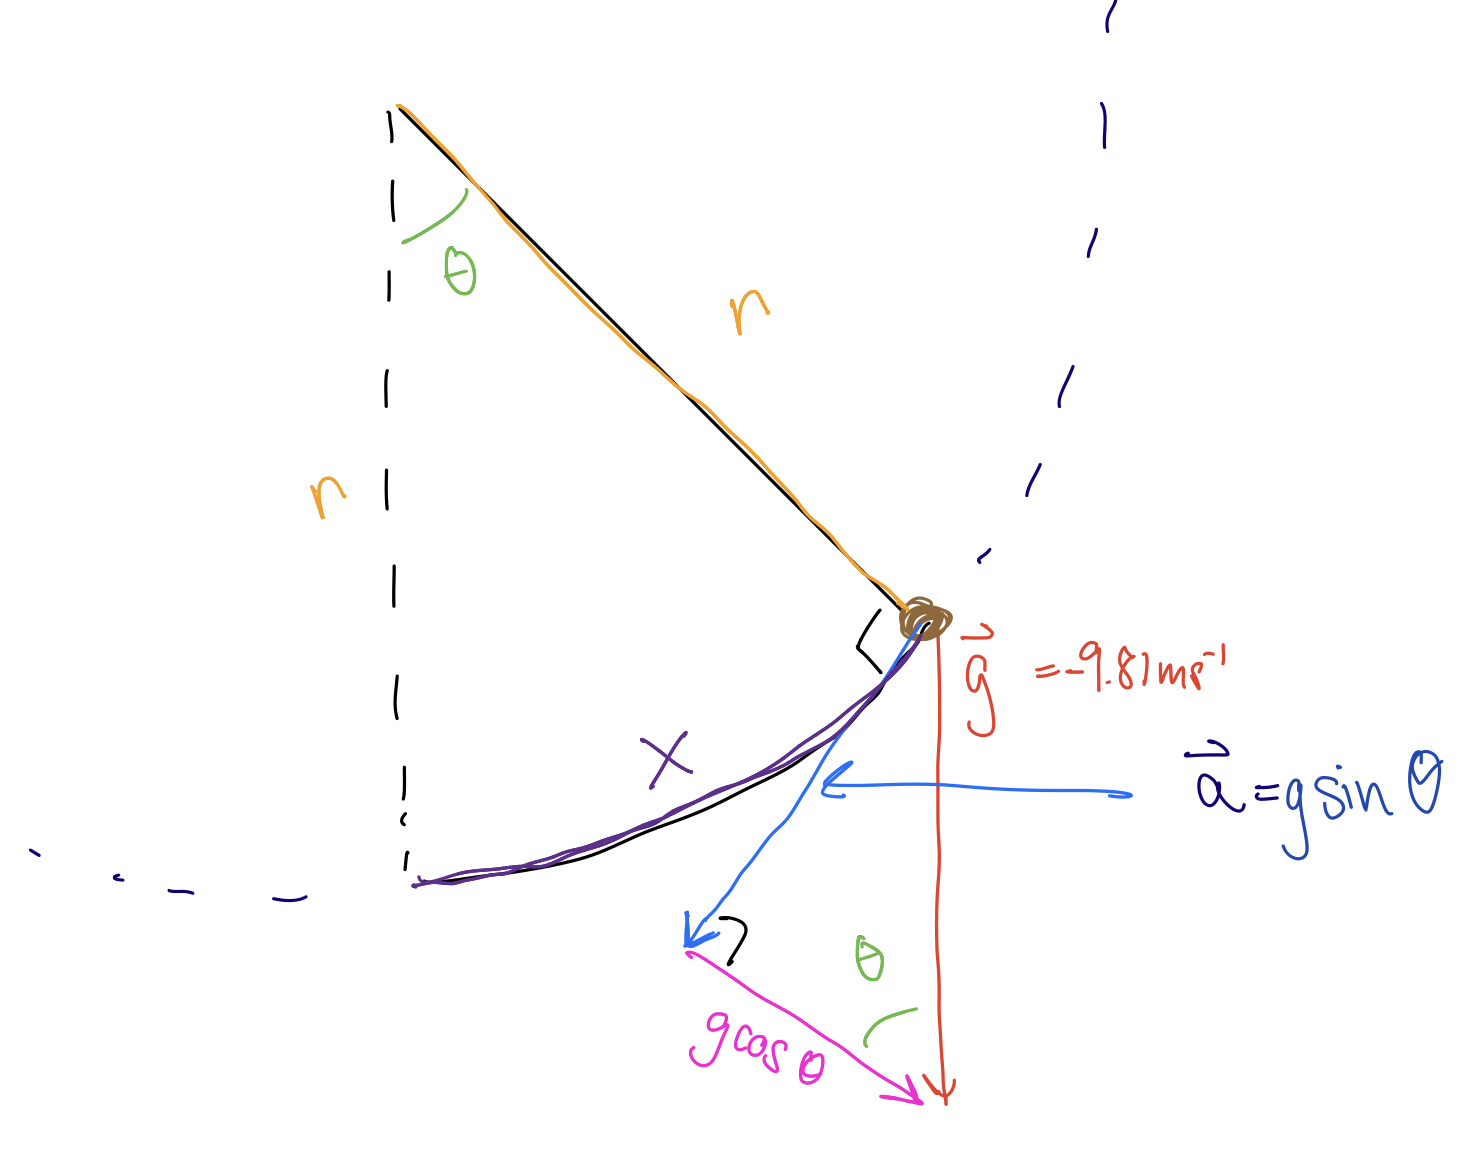
\includegraphics[scale=.45]{acceleration.jpeg} 
\caption{Visualization of Vectors}
\end{center}
\end{figure}

This diagram is a visual depiction of the properties of a pendulum.  From this, the equation for its motion can be determined.  Given an angle $\theta$,  the distance from the center $x$ can be written as $r*\theta$ where $r$ is the radius or length of the pendulum.  A useful vector is the force of gravity on the object.  This can be written as $mg$,  or for simplicity sake,  the diagram denotes the acceleration $g$, equal to $9.81 ms^{-2}$.  However,  the centripetal force (in this case the tension force) constrains the motion of the pendulum.  So in this case,  it is necessary to find the component of gravitational acceleration in the direction tangent to the circle.  Now,  easy geometry can be leveraged to prove that the angle of the pendulum is equal to the angle made by the vectors in the bottom corner (specifically the use of two sets of parallel lines).  Hence,  using SohCahToa with the angle $\theta$,  it is easy to determine that the 'vertical' component of the gravitational acceleration vector is $g \sin(\theta)$.  Giving the angle from the center as a function of time like so: (note a dot denotes one instance of a time-derivative)
\begin{align}
\overrightarrow{a} &= g\sin(\theta) \\
\therefore \ddot{x} &= g\sin(\theta) \\
\therefore r*\ddot{\theta} &= g\sin(\theta) \\
\therefore \ddot{\theta} &= \frac{g}{r}\sin(\theta)
\end{align}

So hence in [4],  we have the true mathematical model of a pendulum not undergoing air-resistance or friction.  In its most faithful representation,  a $-\mu * \theta$ term may be added to denote air-resistance.  It is important to note that this is a stupidly difficult non-linear differential equation...  more on that later.
\subsection{Small Angle Approximation}
To achieve real-world results from complex mathematical abstraction often requires a layer of approximation and simplification.  For example,  the equation given in [4] becomes vastly more manageable when it becomes linear.  The obstruction to this is the annoying $\sin(\theta)$ term nested in there.  Luckily enough,  for small enough angles $sin(\theta)$ is well approximated by $\theta$ itself.  There are many ways to justify this assumption.  To outline a few,  the first term of the McLauren series for $\sin(x)$ is x:
\begin{align*}
\sin(x) &= \sum\frac{f^{(k)}(0)}{k!} \\
&= 0(1) + \frac{1}{1!}x+\frac{0}{2!}x^2 + \frac{-1}{3!}x^3... \\
&= x - \frac{x^3}{6}...
\end{align*}
Additionally this limit can be proved: (using squeeze theorem)
\begin{align*}
\lim_{x\rightarrow 0} \frac{\sin(x)}{x}=1
\end{align*}

Either way,  this simplification will allow us to gain insight about how the system evolves over time to a reasonable degree of accuracy.  So for our purposes,  the differential equation [4] becomes linear and simplifies to:
\begin{align}
\ddot{\theta} &= \frac{g}{r}\theta
\end{align}

\section{The Nature of the Solutions}

\subsection{Exact General Solutions}

Calling the non-approximated non-linear differential equation in [4] difficult would be an understatement  Finding the exact solutions is \textit{stupidly complex}.  It is not impossible,  but involves nasty elliptic integrals,  specifically the "Jacobi Amplitude Function." Now I do not claim \textit{at all} to understand anything about these difficult,  non-elementary functions. 
The only thing I know is that they look cool when plotted on the complex plane using domain coloring!

\begin{figure}[h]
\begin{center}
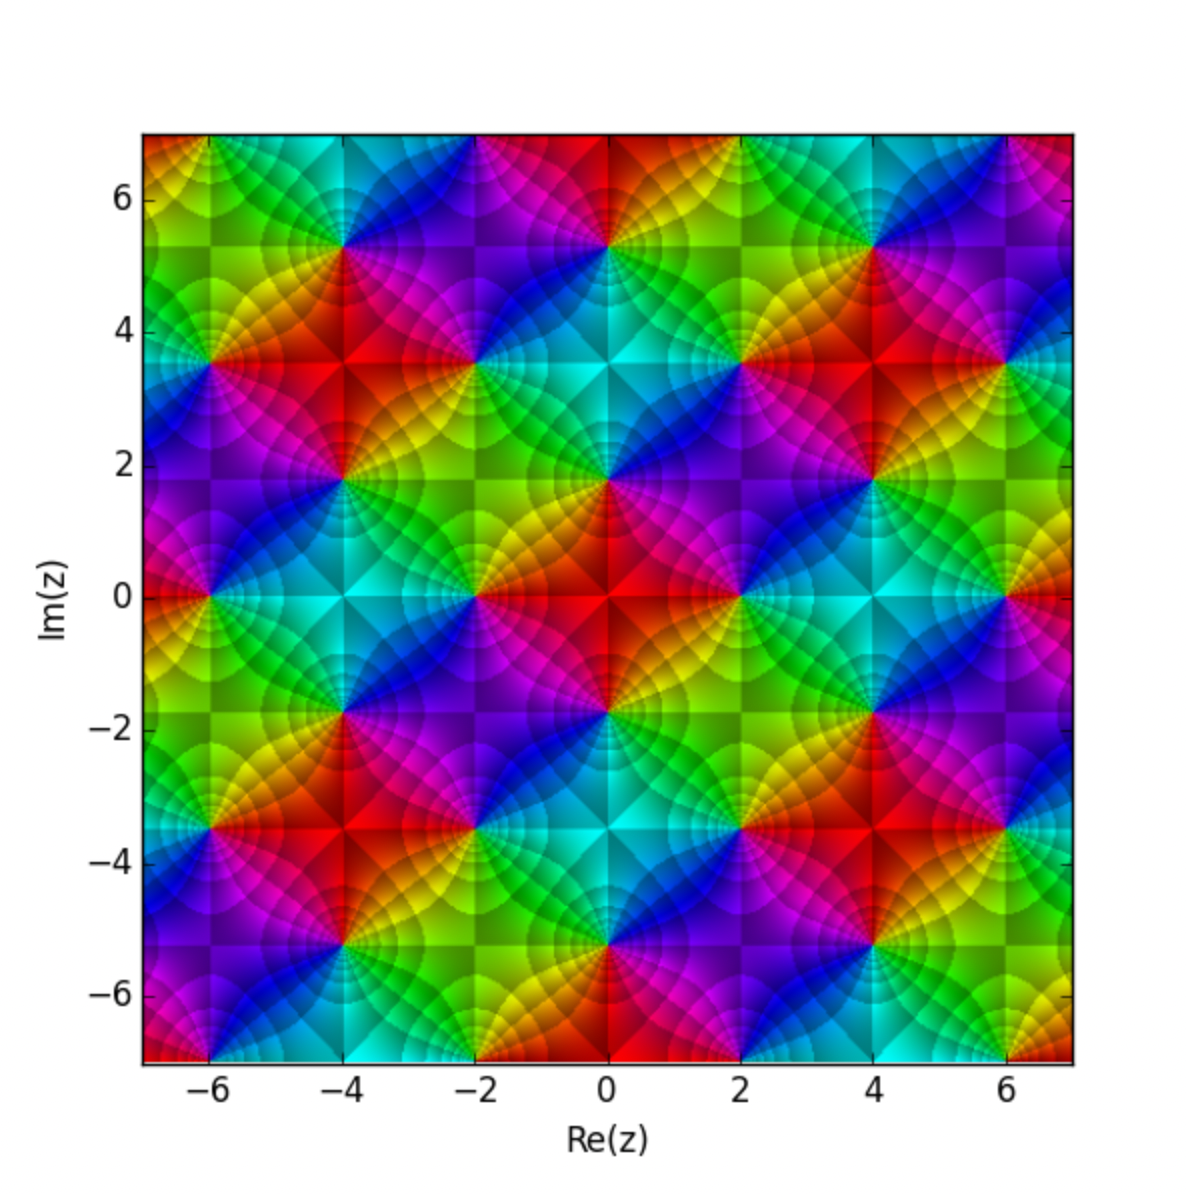
\includegraphics[scale=.4]{cn.png} 
\caption{'cn' Variant of the Jacobi Amplitude Function}
\end{center}
\end{figure}

\subsection{General Solution for Small Angles}

Now,  with the approximation from [5],  this differential equation becomes manageable.  To make the problem more easy to permute,  I will write gravity as $-g$.  So the starting place becomes:
\begin{align}
\ddot{\theta} &= -\frac{g}{r}\theta
\end{align}
And hence can be written as:
\begin{align}
\ddot{\theta} + \frac{g}{r}\theta &= 0
\end{align}
This equation takes the form of a Van der Pol Equation.  These are well-studied and incredibly useful in real world applications.  A famous example is:
\begin{align}
\ddot{y} + y &= 0
\end{align}
Now the nature of these takes the form of a complex exponential (also given that this is non-dampened instance).  So hence $\theta(t) = e^{kt}$ where $k$ is a proportionality constant.  Substituting into [7]:

\begin{align}
\frac{d^2}{d t^2}(e^{kt}) + \frac{g}{r}(e^{kt}) &= 0
\end{align}
Simplifying:
\begin{align}
k^2e^{kt} + \frac{g}{r}e^{kt} &= 0 &\because \text{second derivitive}\\
e^{kt}(k^2 + \frac{g}{r}) &= 0 &\because \text{factor out}\\
k^2 + \frac{g}{r} &= 0 &\because \forall x,  e^x \neq 0 
\end{align}
Solving [12] for k:
\begin{align}
g+rk^2 &= 0 \\
rk^2 &= -g \\
k^2 &= \frac{-g}{r}  \\
\therefore k &= \pm \sqrt{\frac{-g}{r}}\\
\text{or } k &= \pm i\sqrt{\frac{g}{r}}
\end{align}
So from the assumption in [9] we get: (where $c_1, c_2$ are arbitrary constants)
\begin{align}
\theta_1(t) = c_1e^{  i\sqrt{\frac{g}{r}} t},  \text{ and } \theta_2(t) = c_2e^{  -i\sqrt{\frac{g}{r}} t}
\end{align}
An important and useful property of this differential equation is its \textit{linearity}: meaning that a linear combination of any two solutions \textit{is a solution}.  So it follows that the general solution is a linear combination of these solutions:
\begin{align}
\theta(t) = c_1e^{  i\sqrt{\frac{g}{r}} t} + c_2e^{  -i\sqrt{\frac{g}{r}} t}
\end{align}
This is complete,  but it can be expressed in terms of more elementary functions to encode rotation and periodicity instead of complex exponentials. Using Euler's identity that:
\[
e^{i \phi } = \text{cis} (\phi) = \cos(\phi)+ i \sin(\phi)
\]
So hence [19] can be rewritten:

\begin{align}
\theta(t) &= c_1 \text{ cis}  \left(  -\sqrt{\frac{g}{r}} t \right) + c_2 \text{ cis}  \left(  \sqrt{\frac{g}{r}} t \right)
\end{align}
\begin{align}
\theta(t) &=  c_1    \left[     \cos   \left(  \sqrt{\frac{g}{r}} t \right) - i  \sin   \left(  \sqrt{\frac{g}{r}} t \right) \right] + c_2    \left[     \cos   \left(  \sqrt{\frac{g}{r}} t \right) + i  \sin   \left(  \sqrt{\frac{g}{r}} t \right) \right] \\
\theta(t) &= c_1 \cos   \left(  \sqrt{\frac{g}{r}} t \right) - c_1 i  \sin   \left(  \sqrt{\frac{g}{r}} t \right) + c_2 \cos   \left(  \sqrt{\frac{g}{r}} t \right) + c_2 i  \sin   \left(  \sqrt{\frac{g}{r}} t \right)
\end{align}
\begin{align}
\theta(t) = (c_1+c_2) \cos   \left(  \sqrt{\frac{g}{r}} t \right) + i(-c_1+c_2)  \sin   \left(  \sqrt{\frac{g}{r}} t \right)
\end{align}
Now for simplicity,  these constants $c_1,  c_2$ are arbitrary, so they can be redefined for simplicity:
\begin{align}
\textit{Let }\alpha = c_1 + c_2,\textit{ and } \beta = i(-c_1 + c_2)
\end{align}
Hence,
\begin{align}
\theta(t) = \alpha \cos  \left(  \sqrt{\frac{g}{r}} t \right) + \beta \sin  \left(  \sqrt{\frac{g}{r}} t \right)
\end{align}
Now this could be simplified further because of the similarity between cosine and sine,  however this is far enough.

\subsection{Implications}

The primary implication of these general solutions is that a formula for period can be derived.  Now,  [19] alone conveys the period of the function given that the complex exponential function has a period of $2\pi$ as well.  It is arguably more clear,  though,  to show this through the periodicity of $\cos$ and $\sin$.\\ It logically follows that given a sinusoid of the form,
\[A \sin ( \omega t + \phi )\]
$\omega$ denotes 'angular frequency,' measuring angular displacement per unit of time (in radians per second,  ($\frac{m}{ms}$)).  This scalar quantity has a few definitions/applications; the most useful for me is that it is the magnitude of angular velocity.  Regardless,  the most important info to know is that a full resolution is equivalent to traversing an angle of $2 \pi$.  So hence it follows that the time for one complete revolution (a.k.a period) $T$ relates to angular frequency like so:
\begin{align}
\omega = \frac{2\pi}{T}
\end{align}
Now given the general solution in [25] the angular frequency is clearly:
\[ \omega = \sqrt{\frac{g}{r}} \]
Substituting this into [26],  we get the important,  non-trivial identity that:
\begin{align}
\sqrt{\frac{g}{r}} =  \frac{2\pi}{T}
\end{align}
Which mathematically equates gravity,  radius, and period. \textit{(remember only for sufficiently small angles $\theta$)}



\section{Modeling the Problem}

\subsection{Givens}

As outlined in section 1.2,  the given components of this problem are limited in either by usability or accuracy.  The method I chose,  using the angle and the time,  requires the identity in [27] and the assumption that $\sin(\theta) \approx \theta$.  The alternative choice is using visual methods and comparing the approximate size of objects in the frame to the radius.  I opted not to do this, in favor of a more math-oriented option.  \\
To measure the angle from the center,  I used a protractor and determined to a good degree of accuracy that the angle it makes with the vertical is $30$ degrees,  or more applicably $\frac{\pi}{6}$ radians.  It follows as well that the total angle between the two extreme displacements from the center is $\frac{\pi}{3}$ radians.  To maintain a good degree of accuracy when measuring the angle,  I scaled a frame perfect image of the maximum displacement to a large size using the property that angles are preserved when aspect ratio is preserved,  in order to ensure my result was not impacted by human error.\\
The most difficult property to determine accurately is the period.  To mitigate the risk of error,  I used techniques to hopefully minimize the chance of outlines.  I put the video in half-speed and used a stopwatch to measure the time required for the pendulum to complete 5 full periods.  This value was then manipulated by dividing by $2*5$ to correct for the 5 periods and the half speed to get an approximate value for period.  After five iterations of this method,  I averaged the values and determined the time to be $\approx 1.317 \sec$. \\
It is also assumed the pendulum is located close to the earths surface. \\
All the givens are as followed:
\begin{align*}
\theta_{total} &= \frac{\pi}{3} \\
T &= 1.317 s \\
g &= 9.81 ms^{-2}
\end{align*}

\subsection{Determining Radius}

Using the formula derived [27],  it will be permuted to find radius:
\begin{align}
\sqrt{\frac{g}{r}} &=  \frac{2\pi}{T}\\
\frac{g}{r} &=  \frac{4\pi^2}{T^2}\\
r &= \frac{gT^2}{4\pi^2}
\end{align}
Substituting givens:
\begin{align}
r &= \frac{(9.81 ms^{-2})(1.317 s)^2}{4\pi^2}
\end{align}
Approximate answer:
\begin{align}
r \approx 0.431 m
\end{align}
\subsection{Determining Arc Length}

Using the formula for arc length:
\[x = \theta r\]
Substituting givens:
\[x = \frac{\pi}{3} * 0.431003523508... m\]
Approximate answer:
\begin{align}
x \approx 0.451 m
\end{align}

\subsection{Final Answer}
Given all of the quantities determined above,  providing the answer is the easy part.  I will compare the distance covered by the pendulum per unit time to the time in a day.  I will call this 'speed' (note this is \textit{scalar}).  The speed of the pendulum is two times the arc length divided by the period:
\begin{align}
v &= \frac{2x}{T}\\
v &= \frac{2*0.451345834375 m}{1.317 s}\\
v&\approx 0.685 ms^{-1}
\end{align}
Using dimensional analysis to determine the amount of seconds in a day:
\begin{align}
24hr &= 24 hr*\frac{60min}{hr}*\frac{60s}{min} \\
&= 86400 s
\end{align}
Combining these gives the approximate distance the pendulum would cover over one day assuming no friction.
\begin{align}
d &= vt\\
d &= (0.685415086371 ms^{-1})(86400s)
\end{align}
Hence my final answer to three sigfigs is, \textit{the total distance the pendulum would cover over the course of a day would be: }
\begin{equation}
 \approx 59200 \textit{ metres.}
\end{equation}

\section{Reflection on Results}

\subsection{Accuracy of Predictions}

I believe my work reflects a moderate and useful degree of accuracy.  The necessary assumptions made do not impact the outcome significantly enough to skew the results to an unreasonable level.  Within my work provided,  the only major source of error is the simplification of the $\sin (\theta)$ term.  The error caused by this is known,  however.  At the extreme points of the motion,  the value given by $\theta$ will be 4.7\% off: determined by comparing,
\begin{align}
\sin \frac{\pi}{6} &= 0.5 \\
\frac{\pi}{6} &\approx 0.5236
\end{align}
So hence it follows the percent error is:
\begin{align}
&= \frac{|\pi / 6 - .5|}{.5}\\
&= 0.047198\\
&= 4.72\%
\end{align}
Now since this value of theta is larger than the value of its sine as the angle strays from zero,  it means the acceleration will be greater,  and hence the displacement will be greater (this can be proven using the formulas).  Given that this provides an upper bound,  this solution provides the logical inference that the actual result cannot be \textit{too} much lower than the expected values determined. \\

Aside from the accuracy of my work,  the accuracy of my answer is a different question.  Mathematically,  I believe my answer to be strong.  I worked with ample decimal places during calculations and I used an appropriate amount of sigfigs in my answer per the precision of the measurements made.  There are many possibilities of human error as well as inaccuracies in the problem's assumptions.  The lack of givens required me to use a video clip to approximate certain physical quantities.  For example,  it is very possible human error affected my measurement of time despite my attempts to mitigate it.  The significance of an error like this is that it could drastically skew my results.  Similarly,  the limited frame-rate of the video made it difficult to determine the precise angle,  and while I do believe the angle I measured was accurate,  it is possible that it was subject to human error.  Another limitation of my answer is the nature of the question itself.  The question asks us to model the evolution of a short duration action over a long period of time.  The fact that  the answer is over the course of a day means that any small errors in calculation or measurement have the chance of compounding and creating an incorrect and unusable answer.  

\subsection{Context Within the Real World}

Mathematical models of complex systems are innately approximate.  As seen in this problem,  often usable solutions arise out of small simplifications.  A lot of the limitations of a solution is due to the limitations of the measurements.  Aside from this,  the problem makes a drastic assumption that there is no drag force and that the pendulum undergoes simple harmonic motion.  For small angles over a short period of time,  the solution technique provided here will give an answer arbitrarily close to the 'real' value., meaning for all intensive purposes it is a good model of the real world.  However,  adding in major assumptions like the lack of drag forces over long periods of time (relative to the motion of the object) causes the solution to possibly become chaotic and stray far from the real value.  I believe that in this instance,  the simplifying assumptions provide reasonable approximations for the evolution of the system shortly after the initial conditions,  however extending these to longer time periods exasturbates and pronounces the inaccuracies possibly leading to a result that strays from the real value.





\end{document}